\documentclass[12pt,a4paper]{ctexart}
%宏包
\usepackage{amsmath}%数学符号
\usepackage{amssymb}%数学符号
\usepackage{amsthm}%数学符号
\usepackage{geometry}%界面布局
\usepackage{natbib}%bibtex
\usepackage{tikz}%交换图
\usepackage{tikz-cd}%交换图
\usepackage{float}%浮动体固定
\usepackage{caption}%图片标题
\usepackage[colorlinks,linkcolor=blue]{hyperref}%超链接
\usepackage{enumerate}%计数列表
\usepackage{tabularx}%控制列宽

%页面设置
\linespread{1.2}
\geometry{a4paper,left=2cm,right=2cm,top=2.5cm,bottom=2cm}
%\geometry{a4paper,left=2cm,right=2cm,top=2.5cm,bottom=2cm}

%环境和宏指令
\newenvironment{prooff}{{\noindent\it\textcolor{cyan!40!black}{Proof}:}\,}{\par \vskip 1cm}
\newenvironment{proofff}{{\noindent\it\textcolor{cyan!40!black}{Proof of the lemma}:}\,}{\qed \par}
\newcommand{\bbrace}[1]{\left\{ #1 \right\} }
\newcommand{\bb}[1]{\mathbb{#1}}
\newcommand{\p}{^{\prime}}
\renewcommand{\mod}[1]{(\text{mod}\,#1)}
\newcommand{\blue}[1]{\textcolor{blue}{#1}}
\newcommand{\spec}[1]{\text{Spec}({#1})}
\newcommand{\rarr}[1]{\xrightarrow{#1}}
\newcommand{\larr}[1]{\xleftarrow{#1}}
\newcommand{\emptyy}{\underline{\quad}}
\newenvironment{enu}{\begin{enumerate}[(1)]}{\end{enumerate}}
%ctrl+点击文本返回代码  选中代码 ctrl+alt+j 为代码查找文本

%定理环境
\theoremstyle{definition}
\newtheorem{defn}{Definition}[section]
\newtheorem{coro}[defn]{Corollary}
\newtheorem{theo}[defn]{Theorem}
\newtheorem{exer}[defn]{Exercise}
\newtheorem{rema}[defn]{Remark}
\newtheorem{lem}[defn]{Lemma}
\newtheorem{prop}[defn]{Proposition}
\newtheorem{nota}[defn]{Notation}
\newtheorem{exam}[defn]{Example}


\begin{document}
\thispagestyle{empty}

\begin{figure}
    
\includegraphics[scale=0.5]{xjtu.png}
    \centering
\end{figure}
\begin{center}
    \Huge
    \textbf{商务人工智能大作业}
\end{center}
\begin{center}
    \Large
    基于Q-learning思想的离线强化学习的败血症诊断
\end{center}
\vskip 7cm 

\begin{flushleft}
\Large
\textbf{组员:}
兰建伟(强基数学2102, 2213512387) \\ 
张旭航(强基数学2102, 2214414968) \\ 
王尔卓(强基数学2101, 2216110069) \\ 
\textbf{学院:} 数学与统计学院   \\ 
\textbf{任课老师:} 林绍波       \\ 
\textbf{时间:} \today          \\
\end{flushleft}


\newpage
\section{数据背景介绍与问题介绍}
\subsection{数据背景介绍}
MIMIC-III(Medical Information Mart for Intensive Care III)
是由麻省理工学院计算生理学实验室构建的一个大型,免费且开放的重症监护室研究数据集。数据来源于Beth Israe1 Deaconess Medical Center的ICU,
时间跨度为2001年6月至2012年10月,涉及 4 万多名病人的健康数据信息。该数据集主要包括人口统计数据,在病床进行的生命体征测量(每小时约 1 个数据点),实验室检查结果,治疗,药物,护理人员工作记录,影像报告,死亡信息(包括院内和院外)等。

MIMIC-III 
数据集共包括 26 张表格,这些表格可以划分为以下四类,为字典信息数据表,患者及其入院情况的信息表,在重症监护病房中收集的患者数据信息表与医院记录系统收集的数据信息表。
MIMIC-III 数据集已被广泛应用于科研领域,为患者结局预测,实体识别等方面的研究和发展做出了贡献。例如,研究者们可以利用该数据集探究药物使用对检验指标的影响,某医疗手段对死亡率的影响等,从而优化临床决策。此外,该数据集还可以用于开发新的医疗电子工具和提高临床信息化水平。

此处使用的数据是文件中已经处理成 MDP 格式的轨迹文件(未进行数据处理,隐私保护,奖励重塑处理),其中样本被分为训练集,验证集与测试集,比例为 $0.7: 0.1:0.15$ ,
总样本量为 $12984+2787+2786=18557$ 。其中数据结构信息分为 
demog, states, interventions, 1engths, \\ times, acuities, rewards,这七类,
分别对应了样本中的所有时刻的人口统计相关属性,所有时刻的医学指标属性,所有时刻的使用药物,治疗时间,所有时刻的病重程度,奖励值(目前数据里面只在轨迹的最后一个 stage 结束时,
用$1$或$-1$表示奖励, 败血症发作$48$小时后,活着为$+1$ ,死了为$-1$)。
数据具有以下两种特点: 序列长度不一致, 具有稀疏奖励函数。
\subsection{问题介绍}
本问题是关于败血症治疗的生存分析,这里我们希望通过已经有的18557个具体样本数据学习出当败血症病人出现症状后该如何进行对应的药物治疗。“使用强化学习的计算模型能够为重症监护室(ICU)的成年败血症患者动态建议最佳治疗方案。临床医生的目标也是 做出治疗决策,以最大化患者获得良好结果的概率。强化学习具有许多理想特性,可能有助于医疗决策。使用强化学习的模型内在设计能够处理稀疏的奖励信号,这使它们非常适合克服与患者对医疗干预反应的异质性以及治疗有效性 延迟显现相关的复杂性。重要的是,这些算法能够从次优的训练示例中推断出最优决策。”
因此我们这里采样强化学习的方法对该问题进行学习。由于此处我们的样本是离线样本,进行学习任务的智能体只能通过学习离线样本而不能从真实的医疗环境交互去直接学习,因此是离线强化学习。离线Q-learning方法是一个目前关于离线强化学习常见的强化学习算法,此处采用这个算法。
\section{算法介绍}
\subsection{强化学习介绍}
首先先了解强化学习的具体概念,强化学习(Reinforcement Learning,RL)是机器学习的一个分支,旨在训练智能体(Agent)在环境中通过试错来学习如何实现特定的目标或最大化某种累积奖励。强化学习的核心思想是智能体通过与环境的交互来学习最优策略,即在给定状态下选择最佳行动以最大化长期回报。这种学习方法不依赖于标注数据,而是利用奖励信号作为指导,使智能体在不断试错中学习如何采取行动。而离线强化学习则是强化学习的一种变体,离线强化学习主要研究如何利用预先收集的大规模静态数据集来训练强化学习智能体。其核心思想是,智能体无需与环境进行实时交互,而是直接从这些静态数据集中学习最优策略。离线强化学习能够充分利用大规模静态数据集,从而避免了实时交互的成本和时间。这两者同样具有四要素:分别为:
\begin{enu} 
\item 智能体(Agent):智能体是执行任务的客体,通过与环境互动来提升策略。它根据当前的环境状态选择合适的行动,并接收环境的反馈。此处的智能体则为等等需要学习到的Q-learning函数。
\item 环境状态(State):在每一个时间节点,智能体所处的环境状态表示了其当前的环境信息。环境状态是智能体做出决策的基础。此处的环境状态则取样本中所有数据的所有时刻的医学指标属性。
\item 行动(Action):在每一个环境状态下,智能体可以采取的动作。行动直接影响环境的状态,并导致环境的反馈。此处的行动则取样本中所有数据的所有时刻的使用药物。
\item 奖励(Reward):环境对智能体行动的反馈,通常是一个数值信号。奖励信号指导智能体调整策略,以最大化长期累积奖励。此处的奖励则取样本中的奖励值。
本次实现Q-learning算法的学习器集合为线性函数(ls),在文件learner.py中给出了ls学习器相关的训练和测试算法。接下来介绍关于Q-learning的原理步骤。
\end{enu}
\subsection{Q-Learning 介绍}
关于Q-Learning 的学习过程, 是先反向学习$Q$函数后学习路径行动, 
其中$Q$函数的自变量是环境状态与行动, 因变量是奖励值。以下是Q-Learning的步骤(此处先满足markov假设):
\begin{enu}
\item 初始化,创建 $Q$ 值表:为所有可能的状态-动作对赋予初始 $Q$ 值。这些初始值通常设为 0 或较小的随机数。 $Q$ 值表用于存储每个状态-动作对的期望回报。
\item 设 $\hat{Q}_{T+1}=0$ ,使用 Q 值更新公式来更新 Q 值表中对应状态-动作对的 Q 值。更新公式通常基于贝尔曼最优方程,形式如下:
$$
Q_t^*\left(s_t, a_t\right)=\underset{Q_t}{\arg \min } E\left[\left(R_t+\max _{a_{t+1}} Q_{t+1}^*\left(s_{t+1}, a_t, a_{t+1}\right)-Q_t\left(s_t, a_t\right)\right)^2\right]
$$
$t$值以从$T$到$0$的顺序从大到小开始迭代,得到$Q$值表。
\item 执行最优策略, 一旦 $Q$值表达到预设条件, 
智能体就可以根据 $Q$ 值表选择最优策略来执行任务。
这通常意味着在每个状态下选择具有最高 $Q$ 值的动作。即通过以下公式选择最佳动作:
$$
\hat{\pi}_t=\underset{a_t}{\arg \max } \hat{Q}_t\left(s_t, a_{t-1}, a_t\right)
$$
    
\end{enu}
采用该算法的原因如下:
\begin{enu} 
\item 离线Q-learning能够在大规模异构数据集上训练高容量模型,从而产生广泛泛化的智能体。研究表明,离线Q-learning算法在扩展到多任务和大容量模型时,表现出强大的性能。
\item 离线Q-learning算法主要依赖于已有的历史数据进行学习和分析,而不需要智能体与环境进行实时交互。这种特性使得离线Q-learning在隐私保护方面具有天然的优势,因为它不需要实时收集和处理用户的敏感信息。
\item 离线Q-learning算法的可解释性相对较强。由于它基于历史数据进行学习,因此可以通过分析历史数据中的状态、动作和奖励信号等,来理解智能体的决策过程。这有助于人们更好地理解和信任智能体的行为。且此处学习器采用线性函数,可通过观测线性函数的系数来判断一些医学指标对动作决策的影响,更具有可解释性。
\item 离线Q-learning算法可以通过重用历史数据来降低计算代价。由于不需要实时与环境交互,因此可以节省大量的计算资源和时间。此外,离线Q-learning还可以利用经验回放等技术来打破数据之间的相关性,提高学习的效率和稳定性。
\item 离线Q-learning算法在稳定性方面表现出色。由于它基于历史数据进行学习,因此可以避免实时环境中可能出现的噪声和不确定性。此外,离线Q-learning还可以利用目标网络等技术来稳定训练过程,防止Q值函数的过度更新和震荡。
\item 在医疗领域,离线Q-learning算法也具有一定的优势。由于医疗数据通常具有高度的敏感性和隐私性,因此离线Q-learning可以在不直接访问患者数据的情况下进行学习,从而满足医疗领域的隐私保护要求。此外,离线Q-learning还可以利用已有的医疗数据来训练智能体,以提供诊断辅助、治疗建议和药物发现等服务。
\end{enu}
于是采用离线Q-learning算法后, 
根据以上的步骤, 
通过(2)步骤的过程设计了
\\ qfunction\_training与offline\_qfunction\_training,
(3)步骤的过程设计了\\ qfunction\_testing与offline\_qfunction\_testing.
接下来是对算法的实现。

\section{实验结果}
\subsection{算法介绍}
本实验的opt由 ‘fea\_mode’, ‘action\_mode',‘num\_stages'和‘algoname'
这四项构成,其中‘fea\_mode'记录了是否采用马尔可夫假设,‘action\_mode'则记录了是否采用动作分解的操作,此处动作分解的意思是学习在第t步学习Q函数时,
将第t步动作相同的分为一类,学习该动作$a_k$对应的$Q_{a_k}$函数,此处$Q_{a_k}$函数的自变量为状态。
非动作分类则是直接以第$t$步的状态和动作选择为自变量,
奖励为因变量训练出$Q$函数。‘num\_stages’
记录了本次实验对象的轨迹数限制,‘algoname’记录了本次实验采用的学习器的种类。在这次实验中,‘fea\_mode’设为满足马尔可夫假设,‘num\_stages'
设为15,‘algoname'则为ls,
分别将‘action\_mode'设为separate和mix,对比这两者哪个性能更好,最终结果如下:

\begin{figure}[H]
    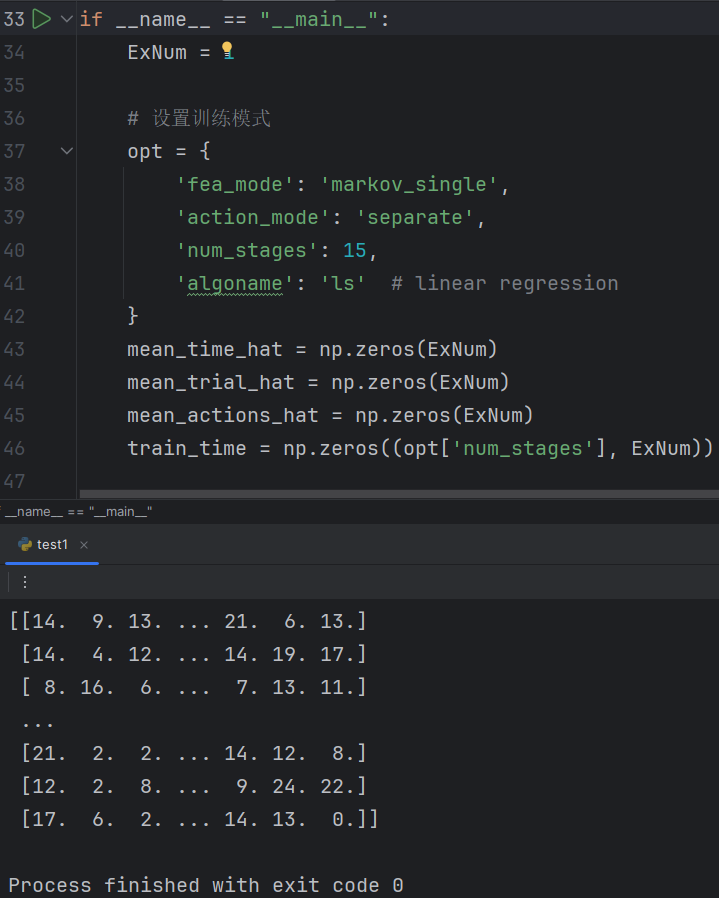
\includegraphics[scale=0.4]{1.png}
    \centering
\end{figure}
\begin{figure}[H]
    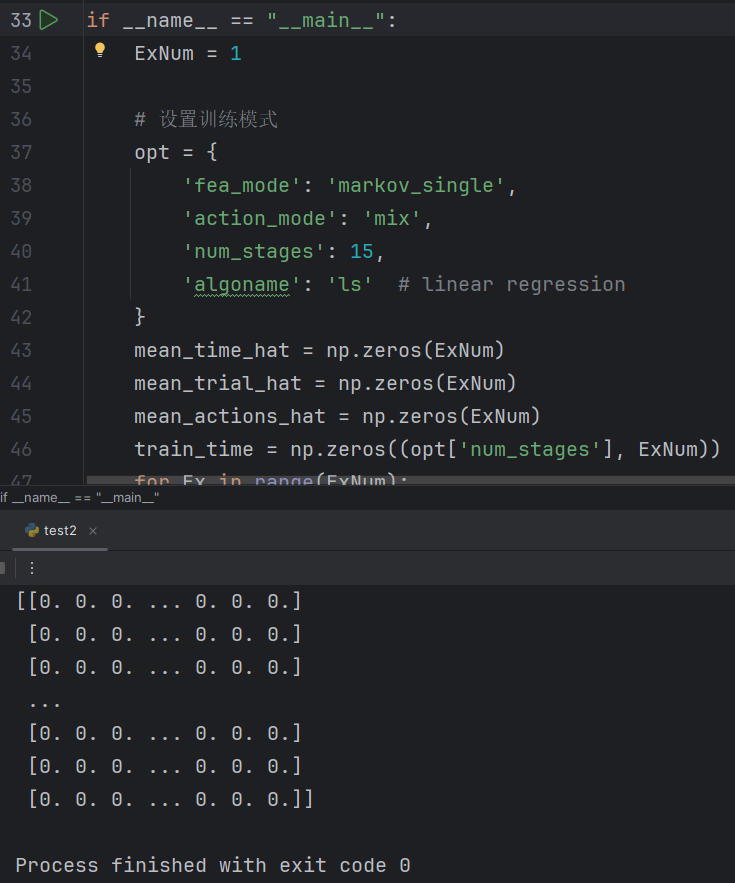
\includegraphics[scale=0.4]{2.png}
    \centering
\end{figure}
\subsection{结果分析}
观测结果,可以得到以下结论:
\begin{enu} 
\item 从输出的结果来看, 
二者都训练出了学习器, 
前者明显对于每个样本都具有个性的输出了不同的药物建议, 而后者对药物使用建议没有区别。
\item separate方法在当前已知的opt条件(马尔可夫假设,ls学习器)
下比mix更具有泛化性。
\end{enu}
实验后, 通过在数学原理上的分析可以得出若在马尔可夫假设下同时采用mix和ls(线性函数)学习器, 
则最终学到的$Q$函数最终量受当前状态和行为的线性影响, 
对于每个个体在最终选择最优动作时是对于每个动作进行遍历而当前状态不变, 
由于学习器是线性函数, 
最终所有个体学习出的动作一定是一致的, 
也就是在这种前提下学习出的结果不具有泛化性。
若最终mix的结果没有那么糟糕, 
需要对比二者的输出结果哪个更好时, 
需要设计一个奖励函数来量化关于输出的优劣, 在没有先验知识的了解下, 
默认存活样本中的每一步对样本的存活影响权重相同, 
得存活样本输出的轨迹行为对应的奖励为$n/m$($n$为轨迹动作重合数, $m$
为原样本总轨迹动作数), 
对应的, 
在没有先验知识的了解下, 
默认死亡样本中的每一步对样本的存活影响权重相同, 
得死亡样本输出的轨迹行为对应的奖励为$-n/m$
($n$为轨迹动作重合数, $m$为原样本总轨迹动作数)。


\section{研究结论}
\begin{enu} 
\item 本次实验成功复现了离线Q-learning算法采用ls学习后对败血症诊断给出了使用药物建议。
\item 本次实验尝试在设置‘fea\_mode’为满足马尔可夫假设,‘num\_stages'为15,‘algoname'为ls的前提下,对动作模式分别为separate和mix的两种方法进行比对,并得出了前者泛化性更好的结论。
\item 从数学理论上分析为什么在马尔可夫假设下同时采用mix和ls(线性函数)学习器不具有泛化性,更清楚的明白了为什么经常将
non\_markov和mix一起设置的原因。

\end{enu}
\par 
代码部分由learner.py, tools.py, test1.py, test2.py, sepsis\_mimiciii
文件夹与\\
sepsis\_mimiciii\_tools文件夹构成,
其中learner存储了学习器种类,tools存储了本次实验所使用的函数,
test1和2是本次实验的运行代码, sepsis\_mimiciii存储了数据,sepsis\_mimiciii\_tools存储了调用数据的函数。


\end{document}